\section{BBC radio production workflow}\label{sec:production}
BBC radio is a huge operation with 59 radio stations spread across the UK
covering every type of programme and music genre. Successfully documenting the
entire system would be difficult if not impossible as different groups and
departments have wildly varying ways of accomplishing the same task.

This section aims to provide a high-level overview of the most common
processes, systems, interfaces and language used in BBC radio production. It
will provide some context to the real-life environment for which the work in
this project will eventually feed into, and may help guide the direction of the
research.

\subsection{Roles}\label{sec:roles}

\paragraph{Producer}
Most radio programmes have one producer who `owns' that programme.  In many
cases, about 80\% of the time spent creating the production is done so by the
producer. In addition to controlling the editorial content, they usually make
the audio recordings and do most of the audio editing. Producers usually only
receive half a day of official training with the rest learnt `on-the-job'.

\paragraph{Presenter/Reporter}
The presenter is the voice of the programme. They provide the links and conduct
interviews with the contributors. In some cases, they work closely with the
producer on the editorial content.

\paragraph{Journalist}
This role is more common in the News division, and the role is usually a
combination of producer and presenter. The emphasis for journalists is on
newsgathering.

\paragraph{Editor}
Editors are senior producers who have a significant amount of experience. They
provide editorial guidance to producers and are often involved with the
programme compliance.

\paragraph{Studio Manager}
The studio manager is responsible for the audio output of the programme. Often
they only get involved at the very end of a production to clean up any rough
edits and apply noise reduction/EQ. In live productions, they operate the
mixing desk and set up remote contributions. In News, senior studio managers
are called Studio Directors.

%\subsubsection{Commissioner}
%When a producer has an idea for a programme, they pitch that idea to a
%commissioner who then decides whether it gets made.

%\subsubsection{Broadcast Assistant}

\paragraph{Media Manager}
Ingests video and audio content for News by setting up ISDN links and BNCS
routing, creating clips from incoming feeds and attaching basic metadata.

\subsubsection{Political structure}\label{sec:organisation}
BBC radio output is produced across three top-level divisions - Radio (formerly
called Audio \& Music), News and North. The structure is listed below.

\begin{itemize}
  \item Radio
  \begin{itemize}
    \item Radio 1, 1Xtra
    \item Radio 2, 6 Music, Asian Network
    \item Radio 3
    \item Radio 4, Radio 4 Extra
    \item Production
    \begin{itemize}
      \item Factual
      \item Arts, Documentaries and Drama
    \end{itemize}
    \item Live Music, Events and Popular Music
  \end{itemize}
  \item News
\end{itemize}

\subsubsection{Services}
The BBC broadcasts a diverse range of speech and music content across genres
including news, drama, comedy, live events, magazine shows, documentaries,
cultural programming and childrens. Quantifying the proportion of these types
of content is difficult as there is little metadata or publications that go
into that level of detail. However, the BBC Trust publishes an annual radio
service
licence\footnote{\url{http://www.bbc.co.uk/bbctrust/our_work/services/radio/service_licences.html}}
which sets aims and objectives for the content of each network. The remits also
include specific conditions which can significantly affect the audio content
(e.g. ratio of music/speech). Using these, it is possible to gauge the
character of each radio network and at least a minimum level of different
content types. The remits and conditions are listed in
Appendix~\ref{app:remit}.

Six of the networks are characterised as a mix of music and speech, with the
other four being purely speech-based. This demonstrates that much more
speech-based audio content is broadcast than music. Of the speech content, much
is likely to be news and current affairs as all of the networks include it to a
greater or lesser extent, and two networks are dedicated to it. With music,
there are a number of conditions that encourage or demand live music and
performances, although the majority of music output will be recordings.

\subsection{Technology}\label{sec:workflow}
The audio workflow at the BBC is vast and complicated. Despite attempts to
harmonise production tools, the wide variety of requirements from production
staff around the BBC means that no one tool can cater for everyone. For
example, some content is turned around in a few minutes whilst other content
could be worked on for a month. However, even though there are plenty of
options available, on a day-to-day basis most producers get by using only the
dira! system.

It would be impractical to capture every single component that audio content
touches at the BBC, so this report will only attempt to detail the most common
systems.  Figure~\ref{fig:workflow} shows a typical audio data flow for radio
production in the BBC.

\begin{figure}[ht]
\centering
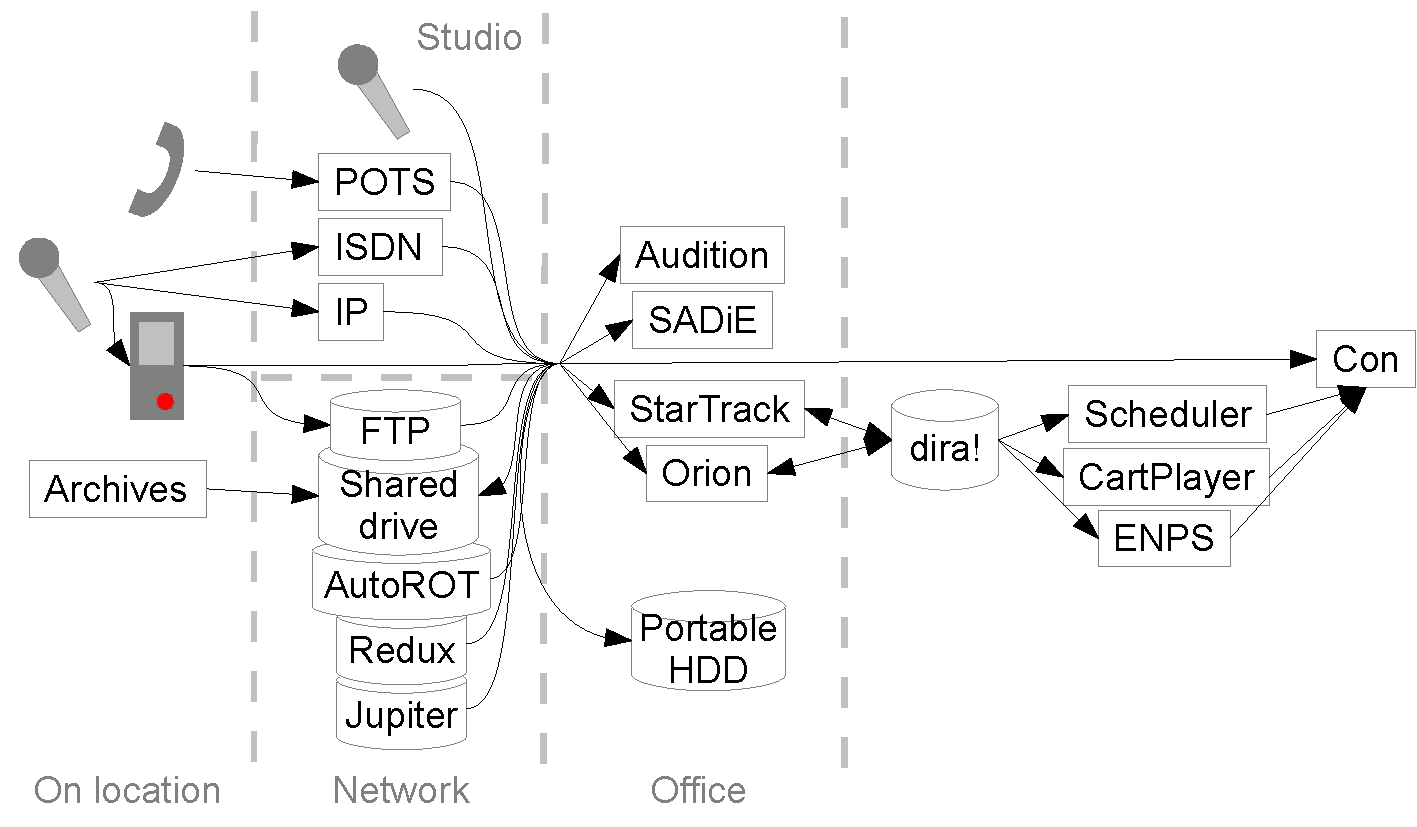
\includegraphics[width=\textwidth]{figs/workflow.pdf}
\caption{Typical flow diagram for audio data in BBC Radio.}
\label{fig:workflow}
\end{figure}

\subsection{Ingest}\label{sec:ingest}
The chosen method of capturing audio content is highly dependent on the type of
programme that is being made. For instance, phone-in shows will combine live
studio recordings with telephone links, and news reports will primarily use
portable recorders. 

\paragraph{Studio recordings}
An obvious but important source of audio content is studio recordings. A
typical set-up consists of an acoustically isolated studio containing a number
of microphones. The studio is connected via triple-glazed windows to one or two
acoustically treated cubicles housing a mixing desk and monitors. The presenter
and guests sit in the studio and the studio manager and producers sit in the
cubicle.

\paragraph{Telephony}
POTS\footnote{Plain old telephone service -- standard phone line} is still used
heavily as it is often the only practical method of setting up remote
contributions on short notice or to members of the public (such as for Radio
4's `Any Answers?' programme).  Where a contribution is planned in advance, an
ISDN\footnote{Integrated Services for Digital Network -- 128kbps digital phone
  connection} link can be set up to a local studio, or to a location equipped
with a ISDN codec box (such as stadiums). This gives a much higher sound
quality but can be expensive if a connection is not already in place.
Increasingly, Internet protocol (IP) links are being used for remote audio
contributions.  Skype is readily used in place of POTS due to its higher sound
quality, and hardware from Comrex (such as its ACCESS and BRIC products) is
being increasingly used to provide high quality contribution links.

\paragraph{Portable recorders}
Recordings made on location are most often made with a microphone and portable
recorder\footnote{Sometimes referred to as a `Nagra' -- a popular brand of
recorder}. The audio, which is stored on Compact Flash or SD cards, is then
either physically taken back to the office or transferred over the Internet
through the use of an FTP server or a browser-based online service provided by
Arbor Media, which automatically copies the recordings into dira!.

\paragraph{Simulrec}
This is a common technique which is used to increase the sound quality of
conversations between a presenter in the studio and a contributor on the
telephone. The interview is conducted over the phone, but each side of the
conversation is also recorded locally using broadcast quality microphones. In
the studio, the recording is made using an audio editor. The contributor is
recorded with a portable recorder and the recording is sent over the Internet
to the studio, where it is imported and lined-up in the audio editor. The
result makes it sound as if the conversation happened in the same room.

\paragraph{Archive} Many programmes require the use of previously-broadcast
material which is stored in one of many archives.

\paragraph{AutoROT} Automatic Record of Transmission (see
Figure~\ref{fig:autorot}) is a popular system that records all network radio
output, plus a number of other streams including the feed from the House of
Commons.  Some of its content stretches back as far as November 2006.  It is
accessed using an online GUI which allows users to audition, clip and download
content.  AutoROT contains a mixture of uncompressed .wav recordings, which are
suitable for re-use, and data-compressed recordings, which are only suitable
for research/browsing.

\paragraph{Jupiter} BBC News store all of their video content in the Jupiter
system, which can be accessed through an online web interface called Davina.
Although not designed specifically for audio content, Jupiter is often used to
take audio data from video recordings.  It is possible to edit audio using a
video editor with Jupiter, but often it is easier to copy the audio content to
dira! and use a program like StarTrack.

\begin{figure}[p]
\centering
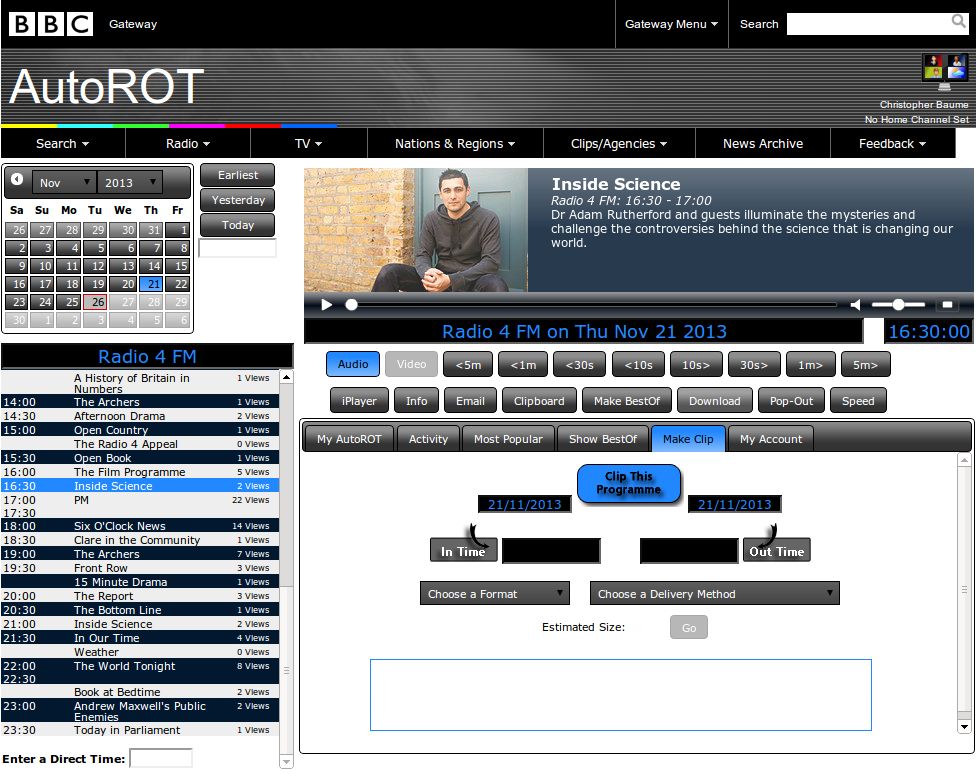
\includegraphics[width=0.8\textwidth]{figs/autorot.png}
\caption{User interface for BBC AutoROT.}
\label{fig:autorot}
\end{figure}

\begin{figure}[p]
\centering
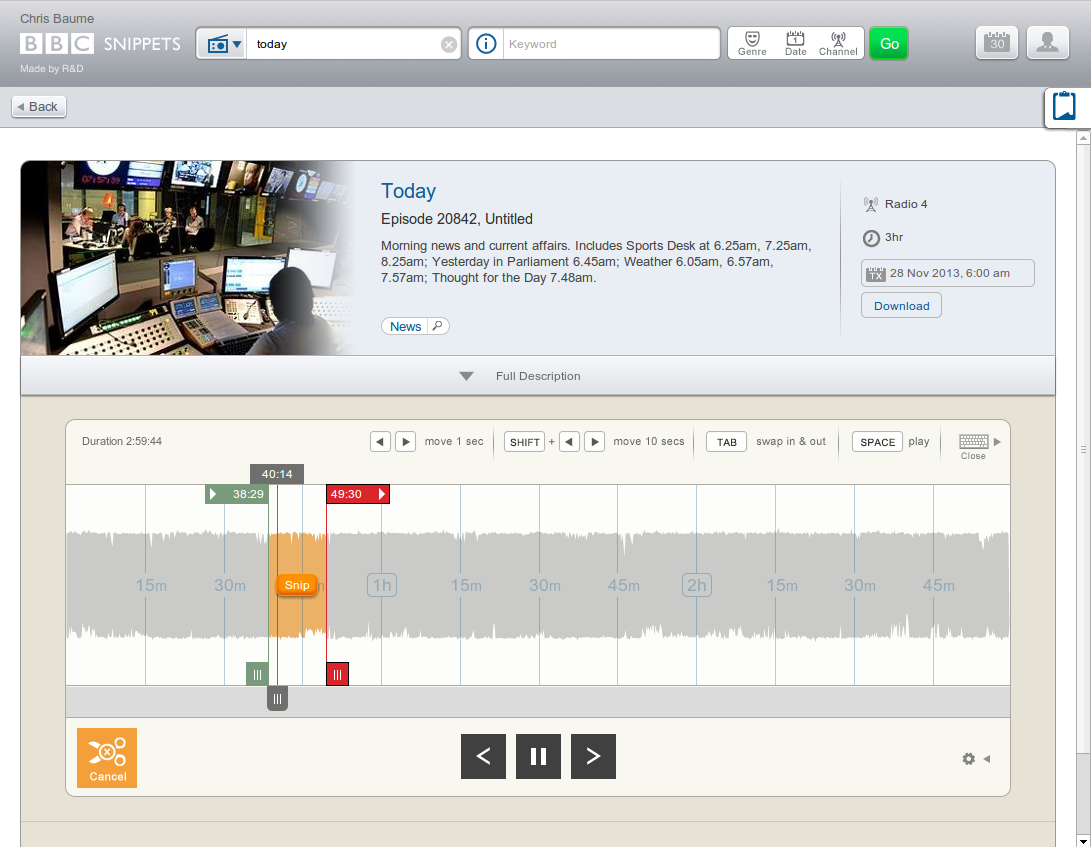
\includegraphics[width=0.8\textwidth]{figs/snippets.png}
\caption{User interface for BBC Snippets for Radio.}
\label{fig:snippets}
\end{figure}

\paragraph{I\&A catalogue}
The BBC's physical archive is managed by the Information and Archives
department, who are primarily based in Perivale. Material can be either be
searched for using the legacy INFAX system or through the new Fabric platform,
both of which are browser-based. Material is found using text-based search
and is then ordered via a phone call. The recording is then either digitised
and deposited in a shared network drive, or the physical media is sent to the
producer via internal mail.

\paragraph{Radio Digital Archive}
The Radio Digital Archive (RDA), and its predecessor the Radio Interim Archive
(RIA), capture all network radio output in uncompressed PCM format. The RIA
started in August 2008 with the RDA taking over in March 2013. They contain
recordings of transmission, pre-recorded items, extended interviews and music
sessions. The RIA stores content as .wav files segmented into 30 or 60-minute
chunks. The RDA uses information from Coyopa (see Section~\ref{sec:coyopa})  to
segment the audio at programme boundaries and to include programme metadata.

\paragraph{Redux}
BBC Redux is an experimental system run by BBC R\&D which records all BBC
television and radio output. It has been running since July 2007. It differs
from other ROT systems in that it records content off-air (via FreeSat). As the
content is data-compressed, it is not fit for broadcast and only used for
programme-making when other archives have been exhausted.

\paragraph{Snippets}
In 2012, a new user interface was developed to allow advanced search and
navigation of Redux. The project, named Snippets, adds features such as the
ability to search the text of television subtitles, audition, clip (`snip') and
download content in-browser and search by cast/crew. The recently introduced
`Snippets for Radio' allows users to navigate radio content with a waveform
display and keyboard shortcuts (see Figure~\ref{fig:snippets}). The code which
powers Snippets for Radio has been open-sourced\footnote{See
  \url{http://waveform.prototyping.bbc.co.uk}}.

\subsection{Storage}

\paragraph{dira! Highlander}
The dira! radio production system is central to the BBC's operation. Almost all
non-live audio content is stored, edited and played out using the system. Dira!
was originally manufactured by a company called \textbf{VCS}, which was then
bought in 2012 by SCISYS. However, within the BBC almost everybody refers to
the dira! system as VCS because of the branding on the software and equipment.

The Highlander program is the user interface for accessing the dira! database
(see Figure~\ref{fig:highlander}). The entire dira! system spans a number of
servers, but Highlander can access only one at a time. Each server consists of
a folder structure where each folder contains a number of `\textbf{stores}'.
The stores contain a `\textbf{take list}' consisting of audio recordings and
StarTrack EDLs\footnote{Edit Decision Lists}.

\begin{figure}[p]
\centering
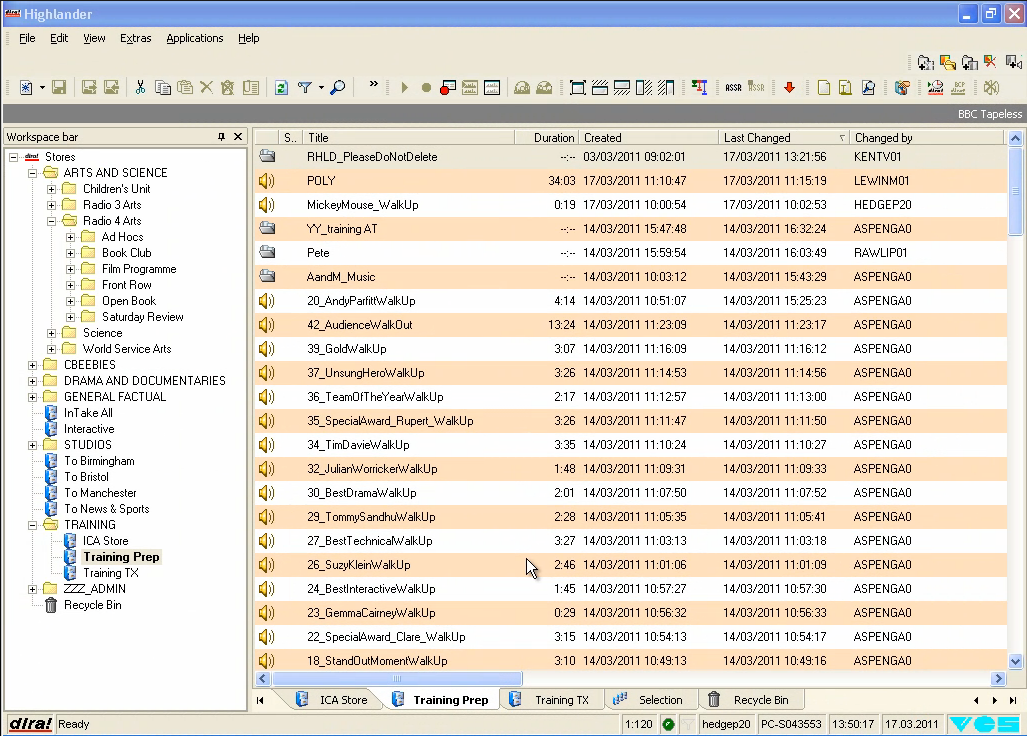
\includegraphics[width=0.9\textwidth]{figs/highlander-interface.png}
\caption{User interface for dira! Highlander.}
\label{fig:highlander}
\end{figure}

Although the stores are technically identical, they are manually arranged to be
used for different purposes, such as:
\begin{itemize}
  \item \textbf{Programme stores}, for regular programmes (such as Woman's
    Hour)
  \item \textbf{Generic stores}, for other programmes in a given network (such
    as Radio 2)
  \item \textbf{Music stores}, for storing music tracks
  \item \textbf{Recording stores}, for raw studio recordings, recordings of
    transmission and presenter links
\end{itemize}

Each store has an individual capacity and expiration time, after which items
are moved to a `\textbf{recycle bin}'. The recycle bin has a 72 hour expiry
time, after which items are unrecoverable. The capacity/expiration parameters
vary for each store, depending on its use. For instance, stores for regular
programmes expire after 30 days, whilst the music stores never expire.

\begin{figure}[p]
\centering
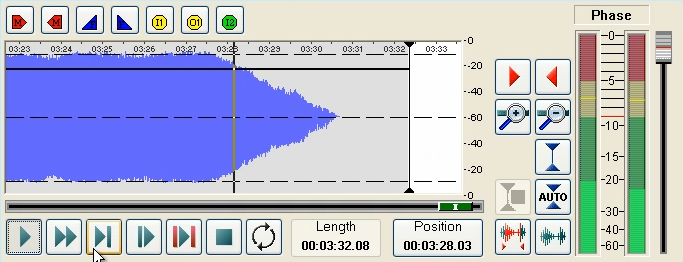
\includegraphics[width=0.9\textwidth]{figs/audition-interface.png}
\caption{User interface for dira! Highlander audition window.}
\label{fig:highlanderaudition}
\end{figure}

Each audio item has a yellow speaker icon which brings up an audition window
(see Figure~\ref{fig:highlanderaudition}) for playing and navigating the clip.
No editing facilities are provided, but there is a button for sending the audio
clip to the StarTrack editor.

Edit decision lists (EDLs) have a folder icon with the letter `A' associated
with them. When selected, they can be opened with the `send to editor' button.

\begin{figure}[p]
\centering
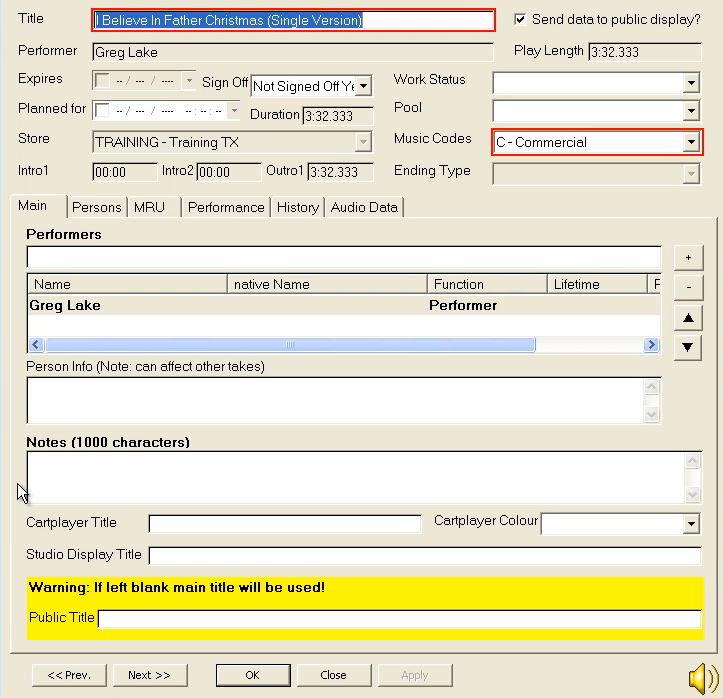
\includegraphics[width=0.8\textwidth]{figs/take-data-card.png}
\caption{Take data card window in dira! Highlander.}
\label{fig:takedatacard}
\end{figure}

Double-clicking on an item opens the `\textbf{take data card}' or `TDC' (see
Figure~\ref{fig:takedatacard}) which is used to read and enter metadata. Some
fields are compulsory and are highlighted in red, and the others are filled in
subject local conventions. There are different types of TDCs for different
types of content. Those which store audio content are called `\textbf{DIGA}s'. 
% explain what EXTA is

\begin{figure}[p]
\centering
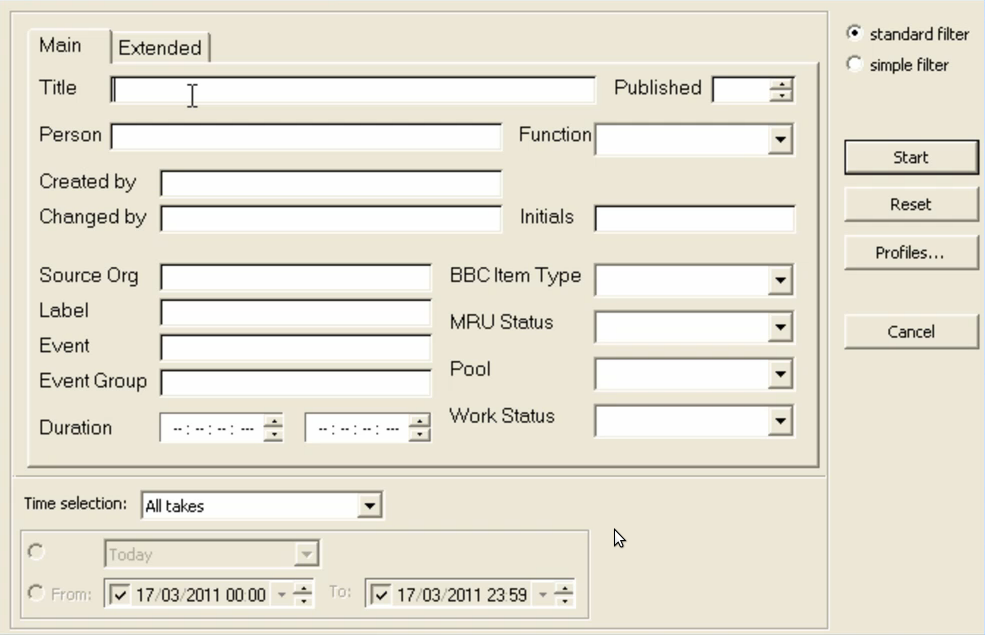
\includegraphics[width=0.8\textwidth]{figs/highlander-filter.png}
\caption{Take list filter window in dira! Highlander.}
\label{fig:highlanderfilter}
\end{figure}

Items can be found by browsing the take list, which can be sorted by title,
duration, time of creation/last modification and username of creator/last
modifier amongst others. The items in the take list can be filtered by text
search, including wildcards (see Figure~\ref{fig:highlanderfilter}), or the
whole server can be searched at once with the results appearing in a separate
window.

\begin{figure}[p]
\centering
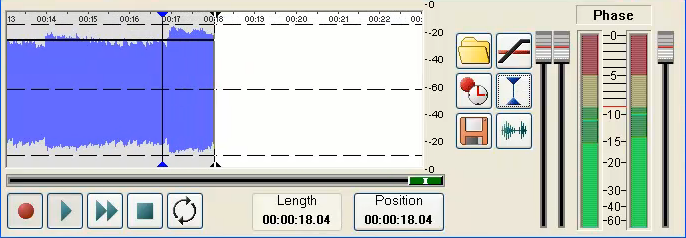
\includegraphics[width=0.8\textwidth]{figs/ats-recorder.png}
\caption{The user interface for ATS recorder in dira! Highlander.}
\label{fig:atsrecorder}
\end{figure}

Audio can be ingested into Highlander by importing a file, making a live
recording or ripping a CD. Imported files are normalised before being uploaded
to the database. The live recordings are made using the `\textbf{ATS recorder}'
program. The interface (see Figure~\ref{fig:atsrecorder}) includes a VU meter,
simple faders, and a button for creating markers. CDs can be extracted using
the CDExtract program, which automatically grabs the CD metadata from an
external database.

\paragraph{Shared network drive}
Audio content is often stored in Windows network fileshares which are mounted
as part of the standard IT infrastructure. Until recently, audio content was
stored in a share mounted as `M:' and known as the `M drive'. This has recently
been replaced with a share mounted as `S:'. The `S drive' is is a disaster
recovery server whose data is split across three sites. Broadcast critical
audio content stored in dira! is automatically copied to S: so that it can be
used if the dira! system fails. However it is also used as a conventional
network drive to store and share content.

\paragraph{Portable hard drives}
Portable USB and Firewire hard drives are popular for transferring and storing
files, despite the risk of data loss. They are often referred to as `Lacie
drives' due to the prevalence of bright orange LaCie-branded drives in the BBC.
Their use is most common when handling large data files which the network can
struggle with, or for storing data when network access is unavailable, such as
on location.

\subsection{Editing}

\begin{figure}[p]
\centering
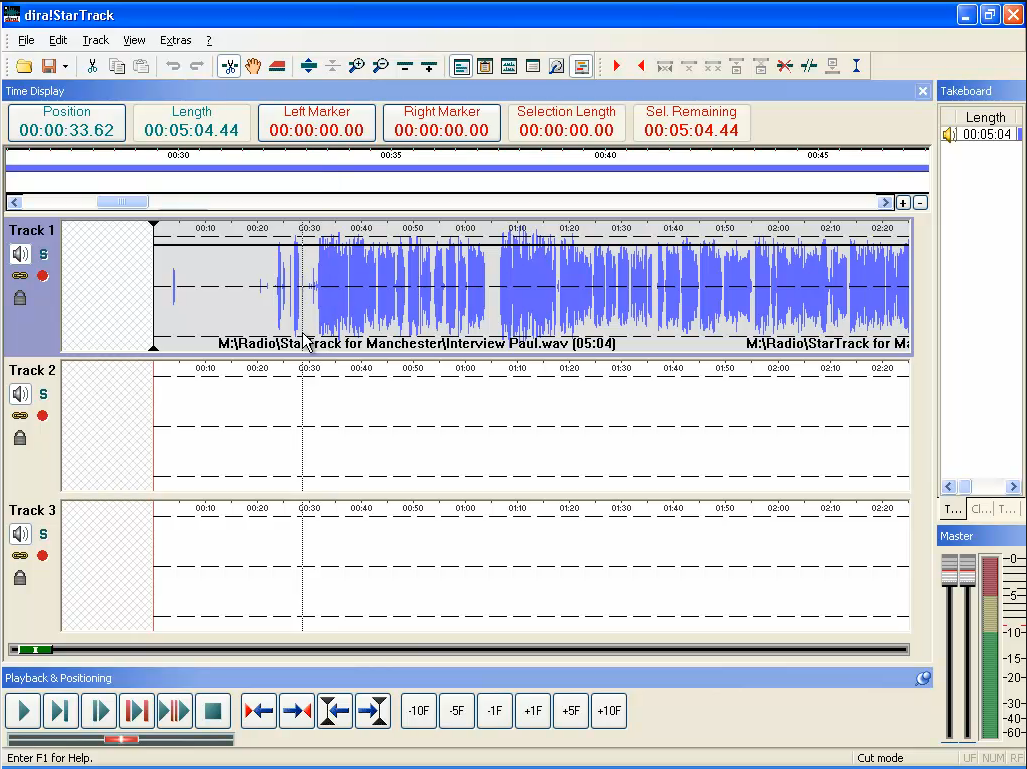
\includegraphics[width=0.8\textwidth]{figs/startrack.png}
\caption{The user interface for StarTrack.}
\label{fig:startrack}
\end{figure}

\paragraph{StarTrack}\label{sec:startrack}
This is widely used throughout the BBC for editing audio content. It is a
multi-track digital audio workstation which provides all the basic editing
facilities a producer would normally require. It is popular due to its tight
integration with dira! and its simple interface, relative to other DAWs (see
Figure~\ref{fig:startrack}).  StarTrack is limited to 16 tracks and is only
able to handle mono and stereo content.

A detailed description of common operations and how they are achieved can be
found in Appendix~\ref{app:startrack}.

\begin{figure}[p]
\centering
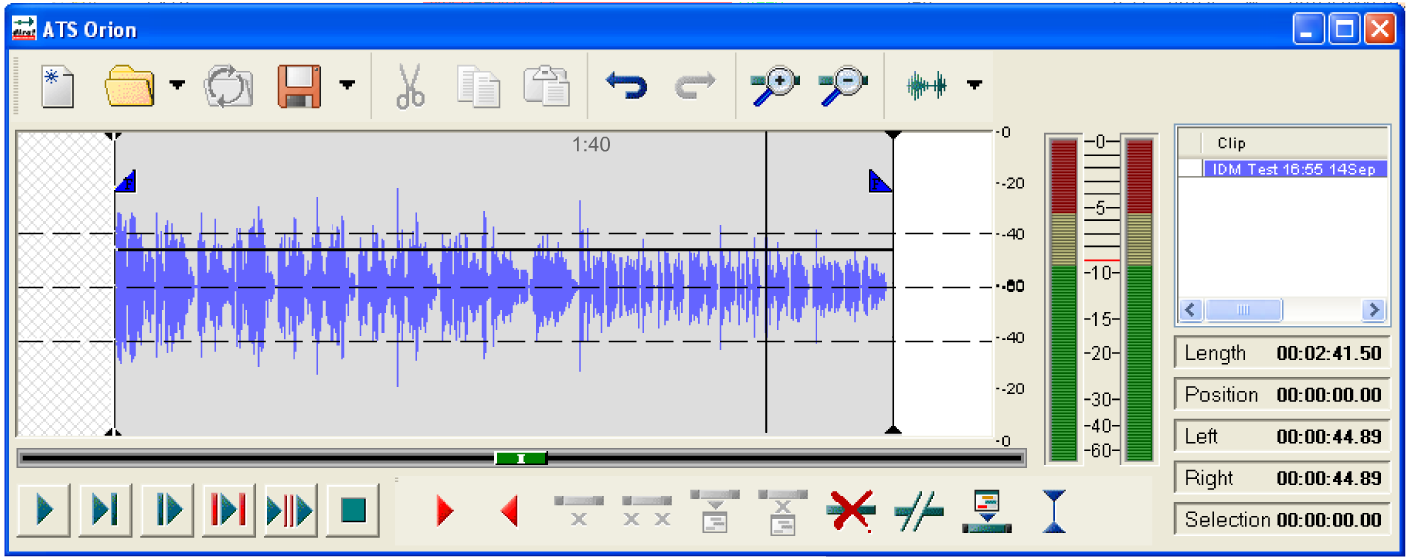
\includegraphics[width=0.8\textwidth]{figs/orion.png}
\caption{The user interface for Orion.}
\label{fig:orion}
\end{figure}

\paragraph{Orion}
This is a single track editor designed for very quick and basic audio edits,
such as level adjustment and top/tailing. It is commonly used within News for
its ability to create clips from incoming live audio feeds as they're being
recorded. Orion is very similar to StarTrack in that it has identical keyboard
shortcuts and includes most of the same features, apart from multiple tracks,
level automation and signal processing, for example.

Notably, when the audio is replayed at greater than normal speed, instead of
playing the samples faster like StarTrack does, Orion skips short segments.
This gives the audio a `choppy' effect, rather than a `chipmunk' effect, but is
more intelligible for some.

\paragraph{SADiE}
This is an advanced digital audio workstation used for more complicated edits
such as for music recordings and documentaries. This is sometimes referred to
as `craft editing'. Certain areas of the BBC, like the Science unit and Radio
3, use SADiE routinely, but in most other areas its use is exceptional.

\begin{figure}[p]
\centering
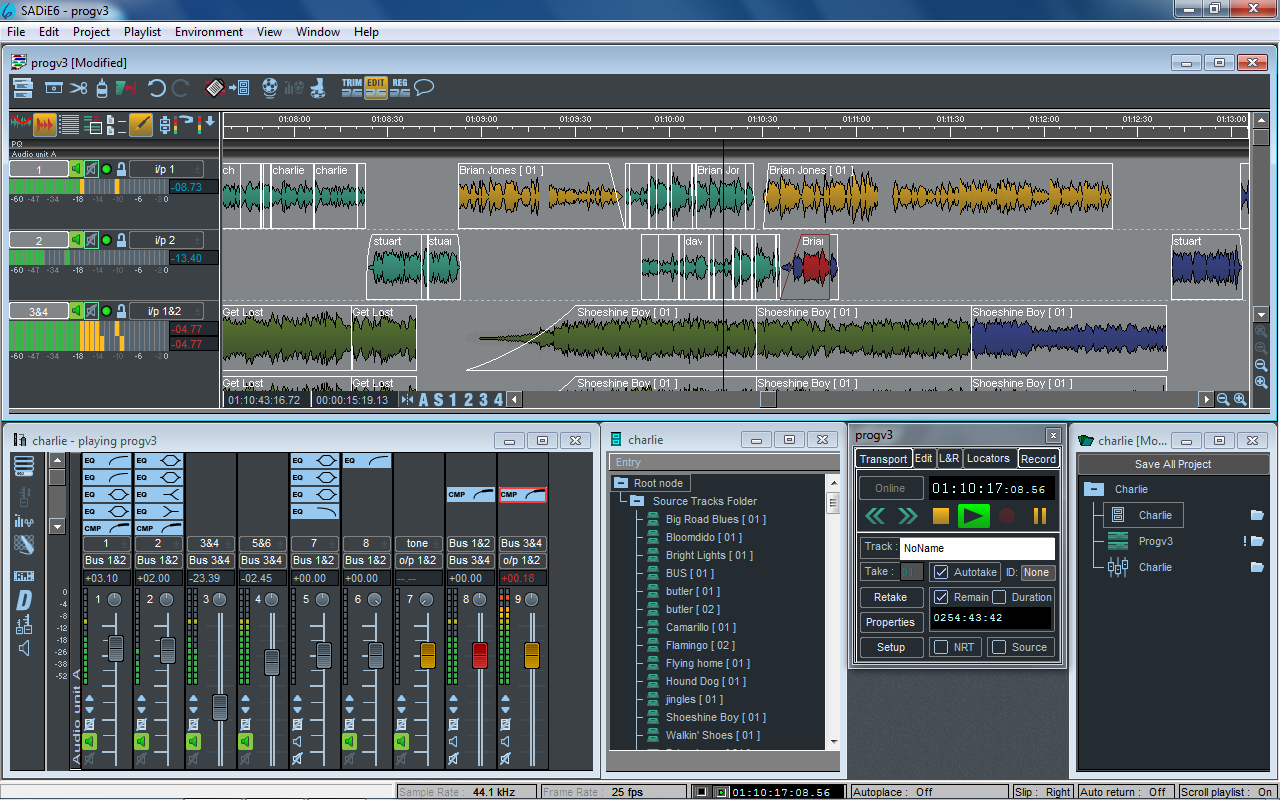
\includegraphics[width=0.8\textwidth]{figs/sadie.png}
\caption{The user interface for SADiE 6.}
\label{fig:sadie}
\end{figure}

SADiE supports a number of extra features not found in StarTrack:
\begin{itemize}
  \item More than 16 tracks
  \item Multi-channel
  \item External audio interfaces
  \item Hardware controllers (e.g. jog wheel)
  \item Larger plugin selection (supports all VSTs)
  \item Channel mixing/routing
\end{itemize}

The interface for SADiE (see Figure~\ref{fig:sadie}) is more complicated, but
is highly customisable and uses a much better waveform renderer.

A plugin package from iZotope is included with SADiE, which included a
multiband compressor, reverb, delay, flanger etc. It also supports all versions
of VST plugins, allowing a much greater selection than StarTrack which only
supports VST v2.0.

\begin{figure}[p]
\centering
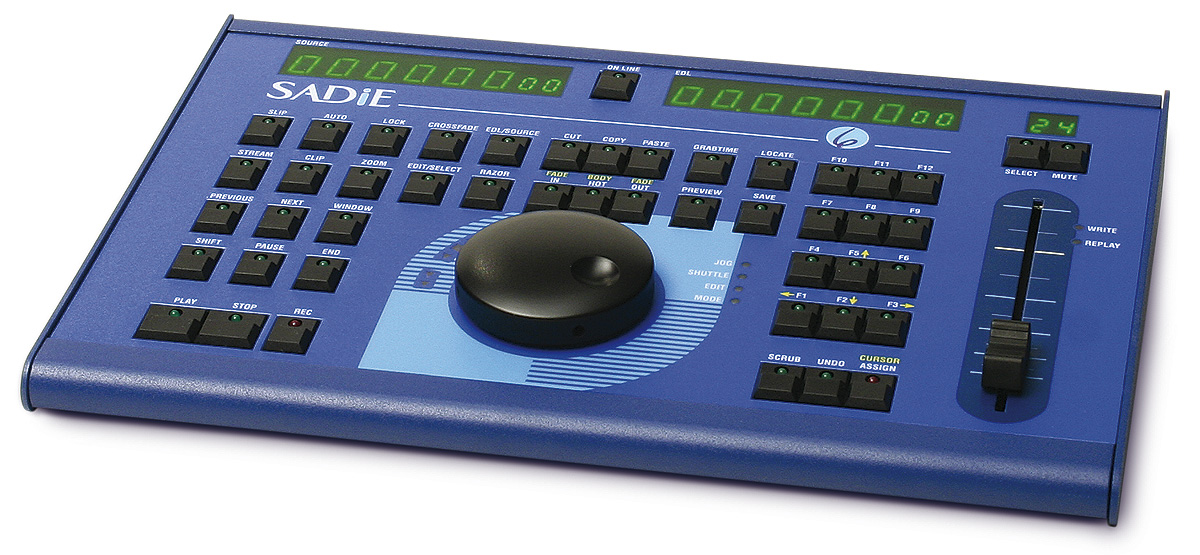
\includegraphics[width=0.8\textwidth]{figs/sadie-controller.jpg}
\caption{A SADiE hardware controller.}
\label{fig:sadie-controller}
\end{figure}

Most common tasks in SADiE can be achieved with its custom hardware controller
(see Figure~\ref{fig:sadie-controller}). These units are common throughout the
BBC and are widely used by those with lots of experience with SADiE. They are
popular because most editing tasks can be achieved more efficiently than with a
mouse and keyboard.

Projects can be converted between SADiE and StarTrack using one of two programs
-- Transporter and SSL Pro--Convert. Although they support basic edits, more
advanced features are not supported, so it is rare for SADiE projects to be
converted to StarTrack.

\paragraph{Audition}
Adobe Audition is used in a similarly way to SADiE, but its use is more popular
in News than Radio. This may be because historically, SADiE workstations could
not be used without dedicated hardware, making them impractical for use
off-site. Cool Edit Pro was used instead, which was then bought by Adobe and
turned into Audition.

\subsection{Metadata}
Metadata is information about data. In the case of radio, it is information
about the audio content. This can include anything from who made a programme to
where particular recordings were made. Collection and use of metadata has
received an increasing amount of attention since the late 1990s as its
importance is recognised. There are two main systems used to collect metadata
on radio productions.

\paragraph{Proteus}
Proteus is a database designed for storing a wide variety of information about
radio programmes. It has been developed by an in-house BBC Radio team since
2001. It can be accessed using a modern browser-based interface (see
Figure~\ref{fig:proteus}). Some of the information it can store includes:
\begin{itemize}
  \item Transmission schedule
  \item Running order
  \item Contributors
  \item Music reporting
  \item Compliance
  \item Descriptions (for iPlayer)
  \item Recordings
  \item Rights
\end{itemize}

\begin{figure}[p]
\centering
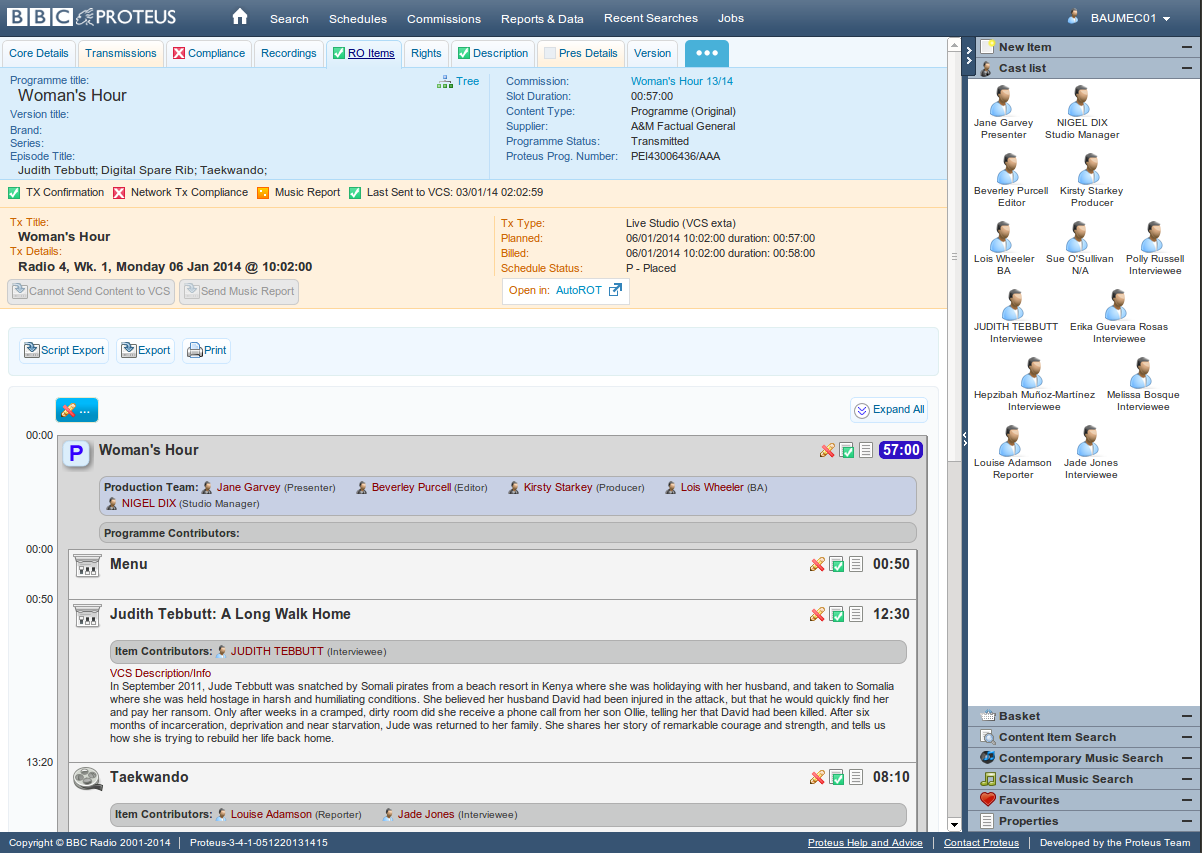
\includegraphics[width=\textwidth]{figs/proteus.png}
\caption{The user interface for Proteus, showing the running order of an
  episode of Woman's Hour.}
\label{fig:proteus}
\end{figure}

There is no requirement to use the system, so different networks and programmes
use the system to varying degrees depending on local convention. Proteus also
duplicates functionality that is found elsewhere, such as music reporting which
can be done in Highlander. 

Each person who uses Proteus does so with a personal account which gives them
different levels of permissions. The system also records the actions performed
by users, which provides version control and audit capabilities. This setup
means that it can be used to co-ordinate approvals for compliance and edit
public-facing information such as the descriptions which feed into iPlayer.

Radio 1, 1 Xtra and 5 Live make minimal use of Proteus as they uses dira! for
music reporting and PowerGold for music rotation. Radio 2 puts presenter
information in, but little else. Radio 3 enters the production team information
and all of the music that is played as its music rotation software relies on
Proteus. Radio 4 uses Proteus more than any major network, particularly shows
such as `You and Yours' and `Woman's Hour', which make full use of the system's
functionality. 

Proteus can be accessed using an API.

\paragraph{Scheduler}
Scheduler is part of the dira! system and allows producers to create a schedule
of programmes and attach metadata to them. Each `programme slot' stores a list
of `elements' which can include text and audio items. The timing of each
element is managed to help the producer plan the programme length. A music
programme, for example, may consist of a track list of dira! audio items (from
a music store) with textual notes between tracks which the presented can use
either as a script or prompts for items to discuss. 

\paragraph{PIPs}\label{sec:pips}
Program Information Platform (known as PIPs) is a database containing
public-facing metadata on BBC TV and radio programmes. It was originally set up
to supply external listings such as Radio Times, but has expanded to feed
the BBC `/programmes' website and iPlayer. Each episode, series and brand has a
unique ID called a programme ID (or \textbf{PID}) made up of eight letters and
numbers (e.g. The Now Show is \texttt{b006qgt7}).

The information stored in PIPs includes:
\begin{itemize}
  \item Schedule
  \item Descriptions
  \item Images
  \item Segments/tracklists
  \item Links
  \item Keywords
\end{itemize}

Much of the data in PIPs is collected automatically from other systems. For
instance, the schedule, title and descriptions are pulled from Proteus, while
tracklistings are pulled from dira!. Further information can be added/edited
using a system called \textbf{iBroadcast}.


\subsection{Playout}
The majority of radio output is broadcast live from a mixing desk and through
the emission chain. However, pre-recorded items must be played out using
software.

\paragraph{Onair Control}
Onair Control is part of the dira! system and provides an interface for
reliably playing audio stored in dira!. Typically, a studio will have a screen
dedicated to displaying Onair Control. It shows a running order containing
text and audio items. Items are selected and played out using a hardware
control interface. The running order is created using Scheduler. 

\paragraph{CartPlayer}
CartPlayer performs a similar function to Onair Control, but is separate and
designed for playing short segments or `stings'. Each audio item is presented
as a square in a grid on a touchscreen. Items are played out by clicking on the
relevant square.

\paragraph{ENPS}
The Essential News Production System (ENPS) is used throughout News across both
television and radio. It is a networked system designed for creating and
sharing news content using written scripts, video and audio content. The ENPS
product is a collaboration between BBC and Associated Press (AP).

\begin{figure}[p]
\centering
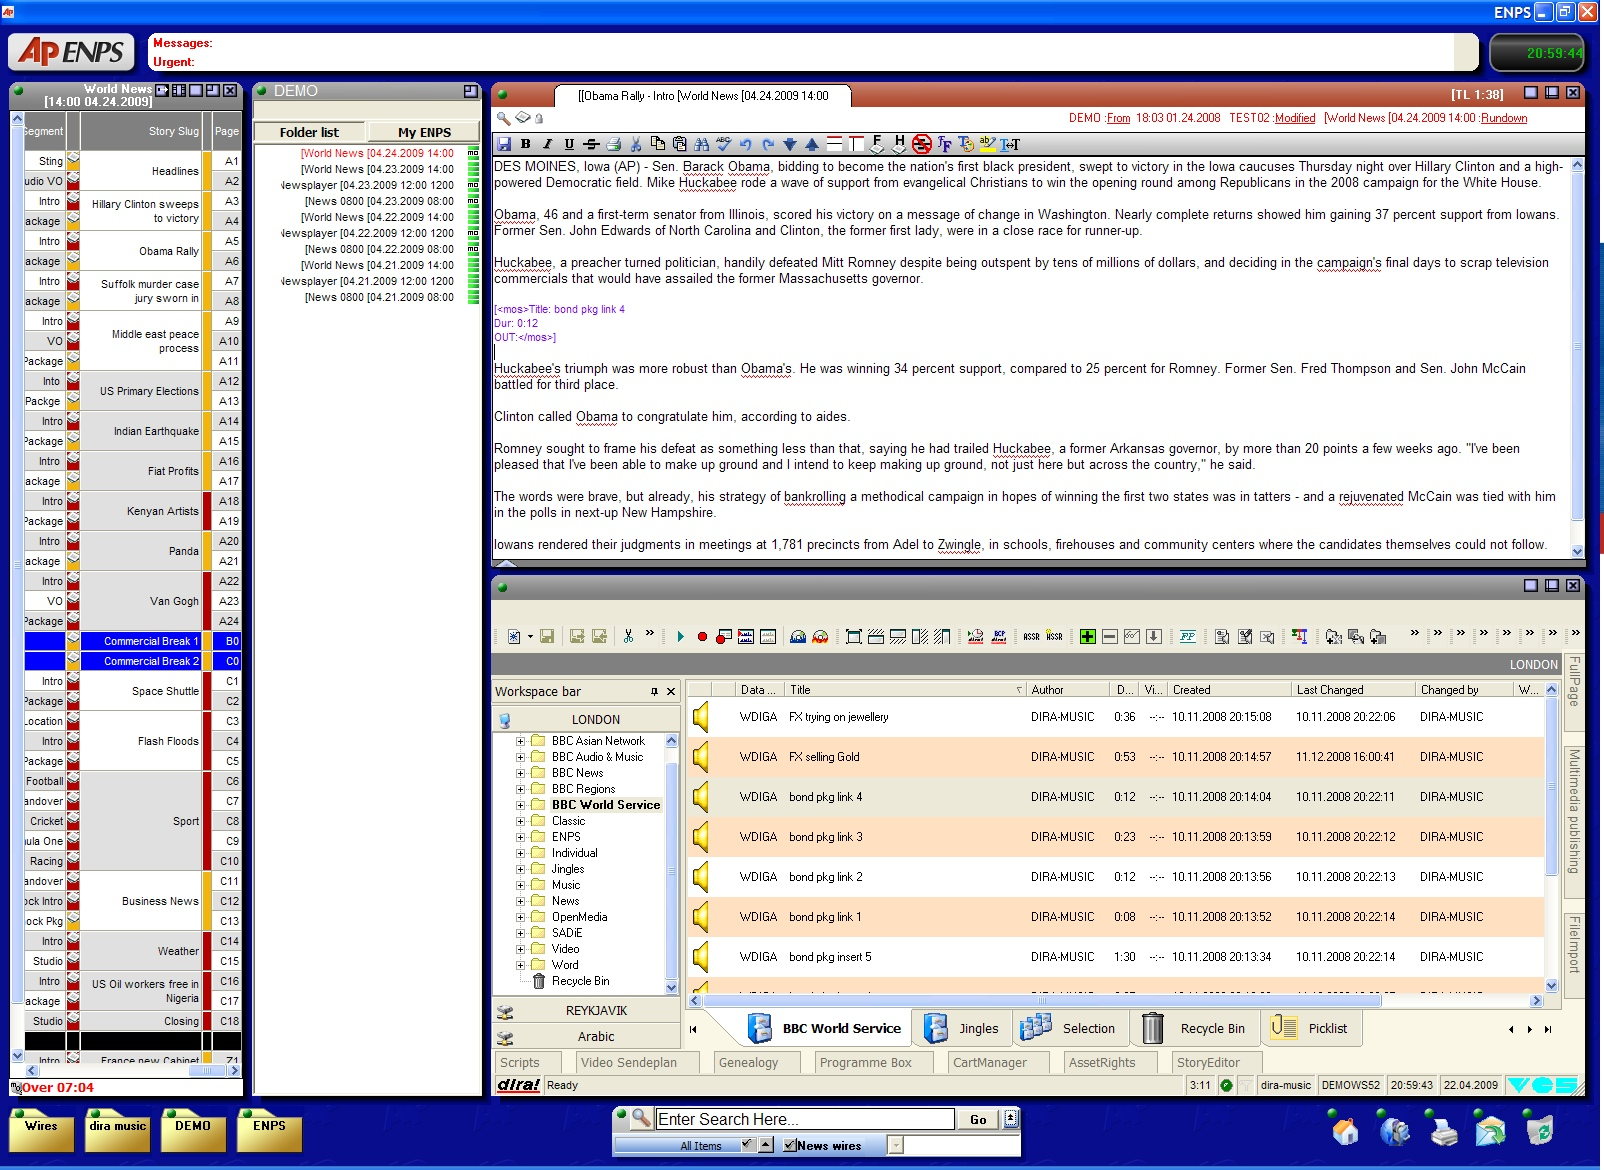
\includegraphics[width=0.8\textwidth]{figs/enps.jpg}
\caption{The user interface for ENPS, including the MOS gateway (bottom right)}
\label{fig:enps}
\end{figure}

The interface (see Figure~\ref{fig:enps}) presents users with a folder
listing and two editing windows, by default. There are four folders to navigate
-- one shared between all news agencies, a personal folder, a programme team
folder and a BBC folder. Folder can contain messages, scripts, running orders
and newsgathering grids. The `MyENPS' feature allows users to create a
customised folder which aggregates different sources. A bar at the top alerts
users to incoming messages and urgent newswire messages.

News content can be found from newswire messages and other sources. Stories are
then written as a script, and video/audio reports can be inserted. Scripts are
arranged into running orders which are used to plan a news programme, including
the time for each segment. When it comes to broadcasting the programme, video
and audio content in the scripts are automatically loaded into the playout
hardware. The presenter reads off the script and the pre-loaded media items can
be triggered at the appropriate time.

The \textbf{MOS gateway} is a plugin to ENPS which allows it to integrate with
dira!. Audio items can be searched for, then drag-and-dropped onto the script.
Those items are then automatically queued for playback.

\paragraph{Coyopa}\label{sec:coyopa}
Coyopa is the BBC's online radio content delivery system, which feeds the
following services:
{\singlespacing
\begin{itemize}
  \item Live streaming
  \item Listen again
  \item Downloads
\end{itemize}
}

The system gets its programme data from PIPs (see Section~\ref{sec:pips}) which
allows it to link what is being played at a particular time to a specific
programme. As the programme is being played out live, the audio content is
encoded using a variety of codecs at different bitrates. This is to allow for
different types of devices (such as PCs, mobile phones and internet radios) to
be catered for.  Coyopa automatically segments programmes at their
boundaries for listen again services, but these can be edited or replaced
afterwards.

\begin{figure}[p]
\centering
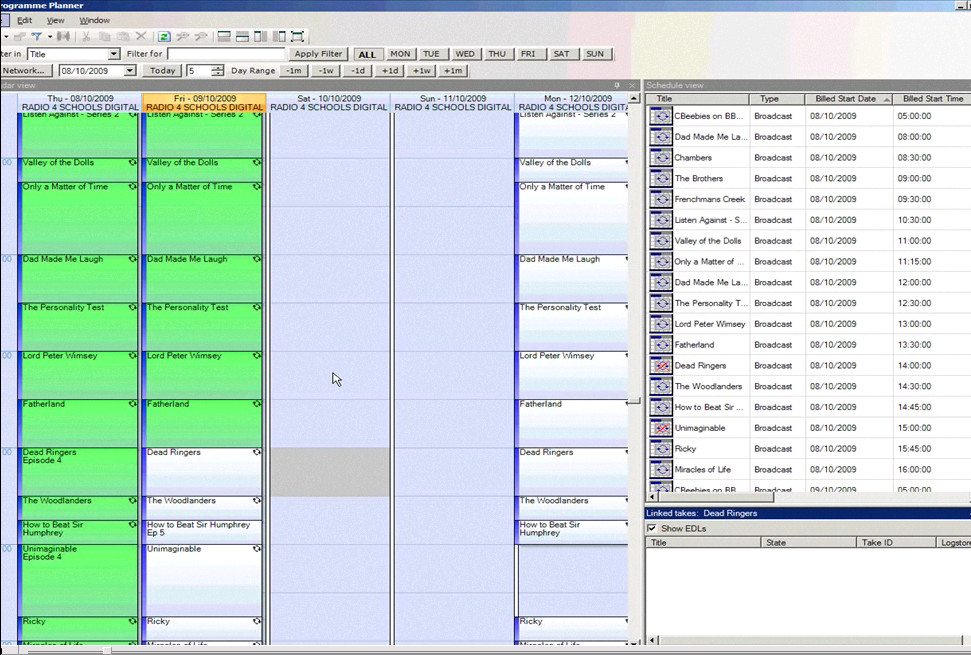
\includegraphics[width=0.8\textwidth]{figs/progplanner.png}
\caption{The user interface for the Programme Planner.}
\label{fig:progplan}
\end{figure}

The \textbf{Programme Planner} is a Windows application which allows the
programme metadata to be edited, and for recordings to be changed. The
interface (see Figure~\ref{fig:progplan}) has both calendar-style and list
views of the programmes. Those that have already been played out are coloured
green. The programme metadata can be edited using the context menu.

Recordings of programmes that have been played out can be edited by
selecting a programme and launching `Coyopa Editor'. This opens an instance of
dira! StarTrack with the automatically-recorded audio content. From here,
producers can top/tail the programme, add an introduction and/or remove content
(for rights reasons perhaps). The programme can also be completely replaced
with a custom recording.

Sensitive content can be blocked in advance using what's called a `live blank'.
This is scheduled for a particular start/end time, and stops content from being
streamed live and being recorded. It can also be set up separately for UK or
international audiences.
